%% SECTION 14C: THE NO-ACCIDENT HORIZON
%% ============================================================
\section{The No-Accident Horizon}
\label{sec:no-accident-horizon}

The strongest form of this paper is not that all future software becomes free. That would be false for arbitrary future programs and misleading for reviewers. The stronger and defensible claim is narrower: once accidental representation, repeated architecture, duplicated contracts, routine behavior families, proof-route discovery, generated-surface drift, dependency rituals, migration folklore, and repair loops have been quotiented away, software converges to a residual floor. That floor is the \textbf{No-Accident Horizon}.

\subsection{The Limit Question}

Let $A_t$ be the admissible software evidence available at time $t$: repositories, issues, pull requests, tests, traces, incidents, vulnerabilities, reviews, schemas, deployment histories, rejected patches, documentation, provenance, license metadata, and rollback evidence. Let $M_t=\canonmap(A_t)$ be the best governed canonical memory produced from that evidence. The memory is admissible only if it preserves provenance, weak-oracle labels, rejected dispositions, security constraints, migration law, and behavior evidence.

Let $Y\sim P_t(Y\mid A_t)$ be a future software demand drawn from a declared workload distribution, and let $\oracle_{\tau,H}$ be an acceptance oracle at evidence tier $\tau$ and future horizon $H$. The oracle includes behavior, hidden compatibility, security, migration safety, provenance, review policy, and future adaptability. A foundry $F$ maps $(M_t,Y)$ to a proof-carrying change object or to a refusal. Its all-in accepted-change cost is
\begin{align}
C_F(Y)={}&C_{\mathrm{intent}}+C_{\mathrm{context}}+C_{\mathrm{reason}}+C_{\mathrm{tool}}
        +C_{\mathrm{verify}} \notag\\
&+C_{\mathrm{review}}+C_{\mathrm{risk}}+C_{\mathrm{amortized\ foundry}}
        +C_{\mathrm{defect}} .
\label{eq:nah-cost-ledger}
\end{align}
The raw baseline $C_{\mathrm{raw}}(Y)$ is the same ledger for the original human repository and process under the same oracle. The denominator is therefore cost per verified correct change, not lines of code, source bytes, prompt tokens, or benchmark solve rate.

For a distribution and oracle, define the removable-work fraction as
\begin{equation}
\Lambda_{\mathrm{NA}}(P_t,\oracle_{\tau,H})
=1-\frac{\inf_{F\in\mathcal{F}_{\mathrm{adm}}}\mathrm{E}_{Y\sim P_t}[C_F(Y)]}
{\mathrm{E}_{Y\sim P_t}[C_{\mathrm{raw}}(Y)]}.
\label{eq:no-accident-horizon-definition}
\end{equation}
The corresponding ideal multiplier is
\begin{equation}
M_{\mathrm{NA}}=\frac{1}{1-\Lambda_{\mathrm{NA}}}.
\label{eq:no-accident-multiplier}
\end{equation}
This normalization is severe. A $10\times$ result means 90\% removable work, a $100\times$ result means 99\% removable work, and a $1{,}000\times$ result means 99.9\% removable work.

\subsection{No Universal Software Inverse}

\textbf{No universal software inverse.} For arbitrary computable programs or adversarial future software demands, no computable foundry has a positive guaranteed No-Accident Horizon. In the distribution-free case,
\begin{equation}
\inf_{P}\,\Lambda_{\mathrm{NA}}(P,\oracle_{\tau,H})=0.
\label{eq:nah-minimax-zero}
\end{equation}

\noindent\emph{Proof sketch.} If a system could always construct, prove, or correctly reject every arbitrary future behavior at finite bounded residual cost, it could decide nontrivial semantic properties of arbitrary programs by encoding those properties as software intents. That contradicts the Turing--Rice boundary~\cite{turing1936computable,rice1953classes,riceTheoremMIT}. If the future distribution is unconstrained, no-free-lunch reasoning gives the learning-theoretic version of the same warning: an optimizer wins only by exploiting non-uniform structure in the task distribution~\cite{wolpert1997nofreelunch}. The shortest adequate description of an arbitrary target is also not generally computable in the Kolmogorov sense~\cite{liVitanyi2008}. A foundry can dominate useful regions of software space, but it cannot own the shortest proof-carrying description of every possible future program.

This negative result is the boundary that makes the positive theory scientific. The claim is not that a model learns all possible future programs. The claim is that economically important software is concentrated in repeated behavior families, organizational patterns, integration rituals, schemas, policies, migrations, operational failures, and product conventions. That concentration is exactly what canonical code exploits~\cite{hindleNaturalness,dejavu2017,jupyterClones2020,clementsProductLines,dreamcoder}.

\subsection{The Horizon Equation}

Normalize today's raw all-in cost mass to one. Decompose it into an irreducible floor $\eta$ and disjoint reducible strata $q_1,\ldots,q_J$:
\begin{equation}
\eta+\sum_{j=1}^{J}q_j=1,
\qquad
q_j\ge 0,
\qquad
\eta\ge 0.
\label{eq:nah-cost-partition}
\end{equation}
Each $q_j$ is a removable source of accidental work: representation search, repository discovery, duplicate truth, proof-lane discovery, invalid edit attempts, routine behavior implementation, generated surface maintenance, retry loops, local architecture reconstruction, dependency rituals, migration folklore, or repeated review reasoning. Let $r_j\ge 1$ be the asymptotic reduction achieved on stratum $j$ by behavior cells, semantic patch cells, proof-carrying changes, canonical profiles, negative memory, renderers, and reusable evidence.

The residual cost fraction is
\begin{equation}
s_{\mathrm{NA}}=\eta+\sum_{j=1}^{J}\frac{q_j}{r_j},
\qquad
M_{\mathrm{NA}}=\frac{1}{s_{\mathrm{NA}}}.
\label{eq:nah-horizon-equation}
\end{equation}
Equation~\ref{eq:nah-horizon-equation} is the Amdahl law of inverse software~\cite{amdahl1967validity}. If two techniques reduce the same failed-search loop, they do not multiply; they compete for the same $q_j$. The exhausted-options limit is
\begin{equation}
\lim_{r_1,\ldots,r_J\rightarrow\infty}M_{\mathrm{NA}}=\frac{1}{\eta}.
\label{eq:nah-final-limit}
\end{equation}
The foundry does not escape the denominator. It drives every reducible term toward zero until only $\eta$ remains.

\subsection{Future-Adaptive Minimum Functional Description Length}

The irreducible floor is not merely source length. It is the cost of new information, acceptance, evidence, governance, and adaptability. An oracle-relative form is
\begin{align}
\mathrm{E}[C_F(Y)]\ge
\mathrm{E}\big[&\alpha K_{\oracle}(Y\mid M_t)
+\beta L_{\oracle}(Y)
+\gamma E_{\tau}(Y) \notag\\
&+\delta G(Y)+\zeta V_H(Y)\big].
\label{eq:nah-info-floor}
\end{align}
Here $K_{\oracle}(Y\mid M_t)$ is the target behavior not already implied by canonical memory, $L_{\oracle}(Y)$ is the description length of the acceptance oracle, $E_{\tau}(Y)$ is the minimum evidence burden, $G(Y)$ is governance and provenance burden, and $V_H(Y)$ is the option-value burden across horizon $H$. This is the \mfdl{} boundary in future-adaptive form: canonicalization can shorten descriptions and make proofs reusable, but it cannot make required new information disappear~\cite{grunwaldMDL,liVitanyi2008}.

\begin{figure*}[t]
  \centering
  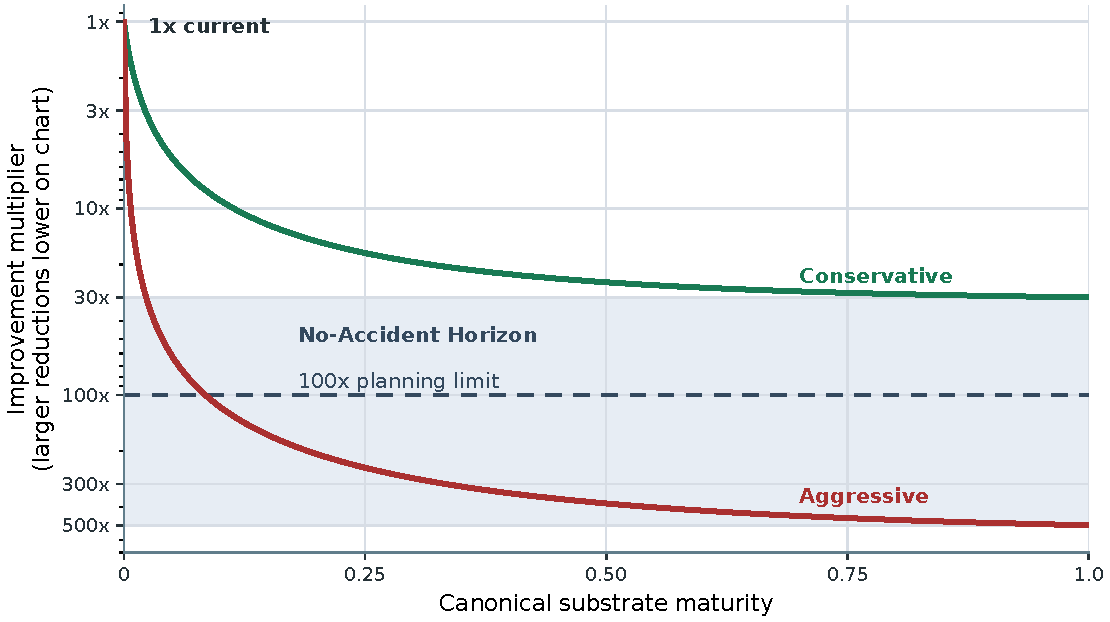
\includegraphics[width=\textwidth]{figures/no_accident_horizon.pdf}
  \caption{Convergence from current all-in verified-change cost toward the No-Accident Horizon. The conservative curve approaches a $30\times$ mature-foundry limit, the aggressive curve approaches a $500\times$ upper-tail limit for supported routine-product work, and the dashed line marks the $100\times$ theoretical planning horizon. The band is a theoretical exhausted-options estimate, not a measured result and not a distribution-free guarantee.}
  \label{fig:no-accident-horizon}
\end{figure*}

\subsection{Numerical Limit Estimate}

The strongest defensible numerical answer is a regime table, not a single slogan. Table~\ref{tab:no-accident-horizon-estimates} states the removable-work fraction $\Lambda_{\mathrm{NA}}$ and reciprocal multiplier $M_{\mathrm{NA}}$ for increasingly favorable assumptions.

\begin{table*}[t]
\caption{No-Accident Horizon: Final-Limit Estimates by Scope}
\label{tab:no-accident-horizon-estimates}
\centering
\footnotesize
\renewcommand{\arraystretch}{1.16}
\begin{tabularx}{\textwidth}{p{0.20\textwidth}X c c c}
\toprule
\textbf{Scope} & \textbf{Interpretation} & \textbf{Conservative} & \textbf{Central exhausted-options limit} & \textbf{Aggressive upper tail} \\
\midrule
Arbitrary programs as mathematical objects & Distribution-free future software, including adversarial and incompressible targets. & $0\%$ / $1\times$ & $0\%$ / $1\times$ & No positive universal bound \\
Broad economically requested software & Product apps plus systems, embedded, data, scientific, security, mobile, infrastructure, creative tools, and genuinely new algorithms. & $75\%$ / $4\times$ & $88\%$ / $8.3\times$ & $96\%$ / $25\times$ \\
Routine product and application software & SaaS, internal tools, resource lifecycles, auth, policy, billing, uploads, jobs, webhooks, audit, migrations, observability, deployment, and integrations. & $96.7\%$ / $30\times$ & $99.0\%$ / $100\times$ & $99.8\%$ / $500\times$ \\
Closed behavior-cell lanes & Narrow lanes where the future change is almost entirely cell selection, parameterization, renderer output, and reusable proof receipts. & $99.0\%$ / $100\times$ & $99.9\%$ / $1{,}000\times$ & $99.98\%$ / $5{,}000\times$ \\
\bottomrule
\end{tabularx}
\end{table*}

The table says three things. First, the universal mathematical problem has no positive guaranteed compression. Second, broad commercial software is compressible but still contains enough hardware, scientific, regulatory, adversarial, organizational, and algorithmic novelty that a universal $100\times$ all-in claim is not defensible. Third, the paper's real frontier is supported routine product software after behavior-genome maturity. In that regime, the strongest defensible final-limit planning number is
\begin{equation}
\Lambda_{\mathrm{NA,product}}^{\star}\approx 0.990
\qquad\Longleftrightarrow\qquad
M_{\mathrm{NA,product}}^{\star}\approx 100\times .
\label{eq:nah-product-star}
\end{equation}
A cautious theoretical band is
\begin{align}
\Lambda_{\mathrm{NA,product}}^{5\%\text{--}95\%}
&\in[0.967,0.998], \notag\\
M_{\mathrm{NA,product}}^{5\%\text{--}95\%}
&\in[30\times,500\times].
\label{eq:nah-product-band}
\end{align}
This is a theoretical limit estimate, not a measured result. It is stronger than the near-term central target because it assumes mature behavior cells, semantic patch cells, reusable proof receipts, negative memory, renderers, and broad amortization. It is weaker than an unqualified $1{,}000\times$ claim because Equation~\ref{eq:nah-final-limit} respects the residual floor.

\subsection{Falsification Rules}

The theory is designed to fail cleanly. Estimate $\eta$, $q_j$, and $r_j$ on paired raw/canonical repositories from the same lineage under the same model, issue distribution, hidden tests, proof lanes, reviewer rubric, and cost ledger. The No-Accident Horizon collapses into ordinary engineering efficiency if any of the following hold:
\begin{enumerate}
\item the irreducible floor $\eta$ remains above $3\%$ for routine product changes after mature canonicalization;
\item behavior-cell and semantic-patch coverage fail to exceed roughly $85\%$ of accepted routine change cost mass;
\item covered strata do not reach at least $100\times$ reduction in context, reasoning, invalid-action, retry, and proof-discovery cost;
\item proof, security, provenance, migration, or review overhead grows enough to erase the saved search cost;
\item canonical ports lose important compatibility ghosts or increase downstream defects at equal review standards;
\item foundry amortization does not compound across independent repositories.
\end{enumerate}
Conversely, the $100\times$ exhausted-options limit becomes conservative if $\eta<0.5\%$, covered routine-change mass exceeds $95\%$, cell-covered strata reach thousands-fold reductions, and proof receipts reuse across many unrelated product lineages without loss of behavior or provenance.

The final claim is therefore precise enough to defend and large enough to matter: the universe of economically important code can be built increasingly close to the No-Accident Horizon, but never beyond it. For arbitrary future programs, the guaranteed horizon is zero. For routine product/application software under a mature behavior-genome foundry, the strongest defensible final-limit estimate is about $100\times$ lower all-in cost per verified correct change, with a cautious $30\times$--$500\times$ theoretical band. Values above $1{,}000\times$ belong to closed behavior-cell lanes where the irreducible floor is below 0.1\%, not to unconstrained software as a whole.

%% ============================================================
